%!TEX root = main.tex
\begin{enumerate}
    \item[A]. Demuestre que para tres variables aleatorias $X$, $Y$ y $Z$ que toman valores sobre conjuntos finitos siempre se tiene que 
    \[
    H(X, Y) + H(X, Z) + H(Y, Z) \geq 2H(X, Y, Z).
    \]
    \begin{proof}
    \textbf{Nota:} Es importante recalcar que todas las variables aleatorias para las cuales se realizan las siguientes pruebas toman valores sobre conjuntos finitos\\
    Para poder probar esa propiedad, primero probaremos lo siguiente, 
    \begin{align}
        H(X,Y,Z)=H(X)+H(Y|X)+H(Z|X,Y)
    .\end{align}
La demostración se tiene a partir de lo siguiente

\begin{align*}
    H(X,Y,Z) &= - \sum_{x,y,z} p(x,y,z) \log p(x,y,z),\\
&= - \sum_{x,y,z} p(x,y,z) \log \left( \frac{p(x,y,z)}{p(x) p(x,y) p(y) p(x)} \right),\\
&= - \sum_{x,y,z} p(x,y,z) \log p(x)  - \sum_{x,y,z} p(x,y,z) \log p(y|x)- \sum_{x,y,z} p(x,y,z) \log p(z|x,y),\\
&= - \sum_{x} p(x) \log p(x) - \sum_{x,y} p(x,y) \log p(y|x) - \sum_{x,y,z} p(x,y,z) \log p(z|x,y),\\
&= H(X)+ H(Y|X)+ H(Z|X,Y).
\end{align*}
De manera análoga tenemos que 
 \begin{align}
        H(X,Y,Z)=H(Y)+H(Y|Z)+H(X|Y,Z)
    .\end{align}
Adicionalmente, tenemos que probar que,
\begin{align}
    H(X,Y)=H(X)+H(Y|X)
\end{align}
Esta prueba se tiene a partir de la siguiente cuenta,
\begin{align*}
    H(X,Y) &= - \sum_{x,y} p(x,y) \log p(x,y) \\
&= - \sum_{x,y} p(x,y) \log \left( p(x) p(y|x) \right)\\ 
&= - \sum_{x,y} p(x,y) \log p(x) - \sum_{x,y} p(x,y) \log p(y|x) \\
&= - \sum_{x} p(x) \log p(x) - \sum_{x,y} p(x,y) \log p(y|x)\\ 
&= H(X) + H(Y|X)
.\end{align*}
de manera similar, se puede demostrar que 
\begin{align}
    H(X,Y)=H(Y)+H(X|Y)
.\end{align}
por último, debemos probar estas dos propiedades
\begin{align}
    H(X|Y)&\leq H(X),\\
 H(X|Y,Z)&\leq H(X|Z)
.\end{align}
Para probar esas propiedades tenemos que usar la convexidad de la función logaritmo cuando tiene base mayor que 1, es decir, que 
\begin{align*}
 \log\left(\sum_{i=1}^{n} \alpha_i x_i\right) \geq \sum_{i=1}^{n} \alpha_i \log(x_i),   
.\end{align*}
donde $\alpha_i > 0$ y $\sum_{i=1}^{n} \alpha_i = 1$; así, $(5)$ se sigue de 
\begin{align*}
H(X) - H(X|Y) &= -\sum_{x,y} p(x,y) \log p(x) + \sum_{x,y} p(x,y) \log p(x|y) \\
&= -\sum_{x,y} p(x,y) \log \frac{p(x)}{p(x|y)} \\
&\geq -\log \sum_{x,y} p(x,y) \frac{p(x)}{p(x|y)} \\
&\geq -\log \sum_{x,y} p(x)p(y) \\
&= -\log(1)\\
&= 0.
\end{align*}
Por lo cual $(5)$ queda probado.\\
Ahora bien, para probar $(6)$ realizamos las siguientes cuentas 
\begin{align*}
H(X|Z) - H(X|Y,Z) 
&= H(X,Z) - H(Z) - H(X|Y,Z) \quad \text{por (3)} \\
&= -\sum_{x,y,z} p(x,y,z) \log p(x,z) + \sum_{x,y,z} p(x,y,z) \log p(z) \\
&\quad + \sum_{x,y,z} p(x,y,z) \log p(x|y,z) \\
&= -\sum_{x,y,z} p(x,y,z) \log \frac{p(x,z)}{p(z)p(x|y,z)} \\
&= -\sum_{x,y,z} p(x,y,z) \log \frac{p(x,z)p(y,z)}{p(z)p(x,y,z)} \\
&\geq -\log \sum_{x,y,z} \frac{p(x,y,z) p(x,z)p(y,z)}{p(z)p(x,y,z)} \\
&= -\log \sum_{x,z} \frac{p(x,z)}{p(z)} \sum_{y} p(y,z) \\
&= -\log \sum_{x,z} \frac{p(x,z)}{p(z)} p(z) \\
&= -\log(1)\\ 
&= 0
.\end{align*}
Así, $(6)$ queda probado. Por lo que, utilizando las propiedades demostradas anteriormente, podemos decir que 
\begin{align*}
    2H(X,Y,Z)&=H(X,Y,Z)+H(X,Y,Z)\\
    &=H(X)+H(Y|X)+H(Z|X,Y)+H(Y)+H(Y|Z)+H(X|Y,Z) \quad \text{por (1) y (2)}\\
    &=H(X,Y)+H(Y,Z)+H(Z|X,Y)+H(X|Y,Z) \quad \text{por (3)}\\
    &\leq H(X,Y)+H(Y,Z)+H(Z|Y)+H(X|Z) \quad \text{por (6)}\\
    &\leq H(X,Y)+H(Y,Z)+H(Z)+H(X|Z) \quad \text{por (5)}\\
    &= H(X,Y)+H(Y,Z)+H(X,Z) \quad \text{por (4)}
.\end{align*}
Concluyendo así, lo que queriamos demostrar.

\end{proof}

    \item[B]. Demuestre que para cualquier tripla de variables aleatorias se cumple que 
    \[
    I(X; Y | Z) = H(X | Z) + H(Y | Z) - H(X, Y | Z).
    \]
    \begin{proof}
    Para poder demostrar esa propiedad, es necesario realizar dos demostraciones preliminares, la primera es probar que para 3 variables aleatorias arbitrarias se cumple que
    \begin{align}
        H(X,Y,Z)=H(X)+H(Y,Z|X)
    ,\end{align}
    esta afirmación se tiene gracias a lo siguiente 
    \begin{align*}
        H(X,Y,Z) &= - \sum_{x,y,z} p(x,y,z) \log p(x,y,z)\\
&= - \sum_{x,y,z} p(x,y,z) \log \left( p(x) p(y,z|x) \right)\\
&= - \sum_{x,y,z} p(x,y,z) \log p(x) - \sum_{x,y,z} p(x,y,z) \log p(y,z|x)\\
&= H(X) + H(Y,Z|X)
    .\end{align*}
La segunda propiedad que tenemos que probar es 
\begin{align}
    I(X;Y |Z) = H(X|Z)-H(X|Y,Z)
,\end{align}
la prueba de esto se sigue de
\begin{align*}
    I(X;Y | Z) &= - \sum_{x,y,z} p(x,y,z) \log p(x,y|z)\\
&= H(X|Z) + \sum_{x,y,z} p(x|z) p(y|z) p(x,y,z) \log p(x|z) + \sum_{x,y,z} p(x,y,z) \log \left( \frac{p(x,y,z)}{p(x,y|z)} \right)\\
&= H(X|Z) - H(X|Y,Z)
.\end{align*}
por lo anterior, podemos decir que 
    \begin{align*}
        I(X;Y | Z) &= H(X | Z) - H(X | Y, Z)\quad \text{por (8)}\\
&= H(X | Z) - \left( H(X, Y, Z) - H(Y, Z) \right) \quad \text{por el numeral anterior y el (3)}\\
&= H(X | Z) - \left( H(X, Y | Z) + H(Z) \right) + H(Y, Z) \quad \text{por (7)}\\
&= H(X | Z) + H(Y | Z) - H(X, Y | Z) \quad \text{por (4)}
    .\end{align*}
\end{proof}

    \item[C]. Proponga una definición para la información común de tres variables $I(X; Y; Z)$ y demuestre que 
    \[
    I(X; Y; Z) = I(X; Y) - I(X; Y | Z).
    \]
    \begin{proof}
    Teniendo en cuenta que $I(X;Y;Z)$ representa la cantidad de información que tienen en común las tres variables aleatorias \( X \), \( Y \) y \( Z \), podemos entender este concepto de manera más intuitiva a través de una perspectiva más conjuntista. Según lo aprendido en clase, sabemos que \( H(X;Y;Z) \) se refiere a la entropía total del sistema, mientras que \( H(X) \), \( H(Y) \) y \( H(Z) \) representan las entropías individuales de cada una de las variables. Por otro lado, \( I(X;Y) \), \( I(X;Z) \) y \( I(Y;Z) \) denotan la cantidad de información común entre dos variables aleatorias.

Si representamos estas relaciones en un diagrama de Venn, podemos ver de manera gráfica cómo se superponen las distintas informaciones y cómo se relacionan entre sí. 


        \begin{center}
            

\tikzset{every picture/.style={line width=0.75pt}} %set default line width to 0.75pt        

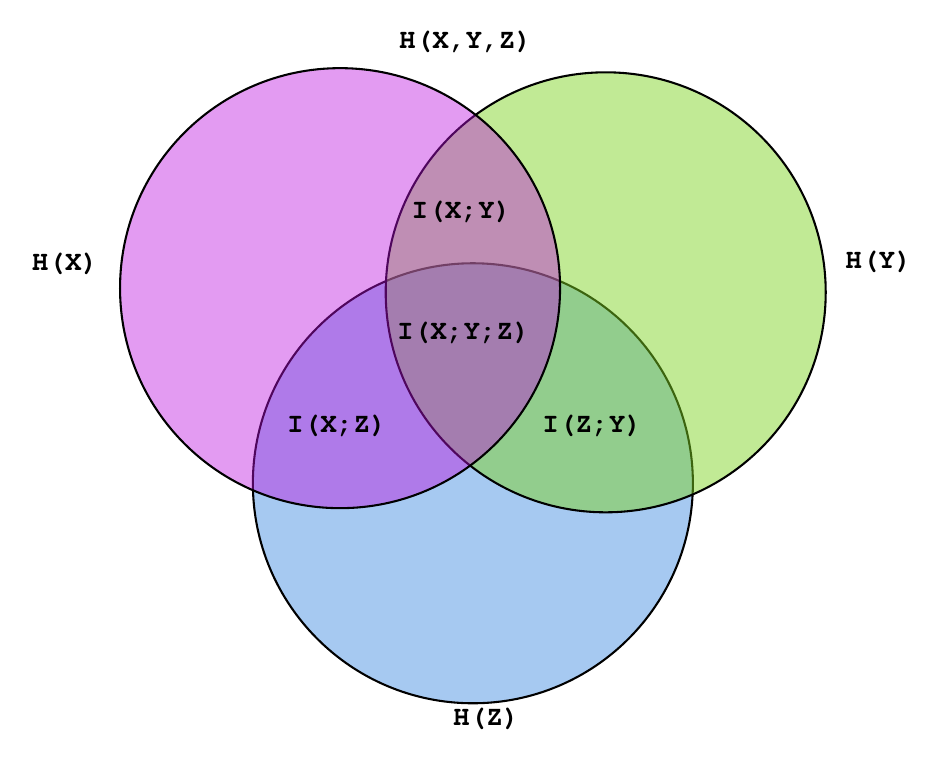
\begin{tikzpicture}[x=0.75pt,y=0.75pt,yscale=-1,xscale=1]
%uncomment if require: \path (0,455); %set diagram left start at 0, and has height of 455

%Shape: Circle [id:dp24857991007765134] 
\draw  [fill={rgb, 255:red, 74; green, 144; blue, 226 }  ,fill opacity=0.49 ] (117,227) .. controls (117,168.46) and (164.46,121) .. (223,121) .. controls (281.54,121) and (329,168.46) .. (329,227) .. controls (329,285.54) and (281.54,333) .. (223,333) .. controls (164.46,333) and (117,285.54) .. (117,227) -- cycle ;
%Shape: Circle [id:dp20129106649070594] 
\draw  [fill={rgb, 255:red, 126; green, 211; blue, 33 }  ,fill opacity=0.48 ] (181,135) .. controls (181,76.46) and (228.46,29) .. (287,29) .. controls (345.54,29) and (393,76.46) .. (393,135) .. controls (393,193.54) and (345.54,241) .. (287,241) .. controls (228.46,241) and (181,193.54) .. (181,135) -- cycle ;
%Shape: Circle [id:dp2743136534598867] 
\draw  [fill={rgb, 255:red, 189; green, 16; blue, 224 }  ,fill opacity=0.42 ] (53,133) .. controls (53,74.46) and (100.46,27) .. (159,27) .. controls (217.54,27) and (265,74.46) .. (265,133) .. controls (265,191.54) and (217.54,239) .. (159,239) .. controls (100.46,239) and (53,191.54) .. (53,133) -- cycle ;

% Text Node
\draw (186,8) node [anchor=north west][inner sep=0.75pt]  [font=\normalsize] [align=left] {{\fontfamily{pcr}\selectfont \textbf{H(X,Y,Z)}}};
% Text Node
\draw (9,115) node [anchor=north west][inner sep=0.75pt]  [font=\normalsize] [align=left] {{\fontfamily{pcr}\selectfont \textbf{H(X)}}};
% Text Node
\draw (401,114) node [anchor=north west][inner sep=0.75pt]  [font=\normalsize] [align=left] {{\fontfamily{pcr}\selectfont \textbf{H(Y)}}};
% Text Node
\draw (212,334) node [anchor=north west][inner sep=0.75pt]  [font=\normalsize] [align=left] {{\fontfamily{pcr}\selectfont \textbf{H(Z)}}};
% Text Node
\draw (185,148) node [anchor=north west][inner sep=0.75pt]  [font=\normalsize] [align=left] {{\fontfamily{pcr}\selectfont \textbf{I(X;Y;Z)}}};
% Text Node
\draw (192,90) node [anchor=north west][inner sep=0.75pt]  [font=\normalsize] [align=left] {{\fontfamily{pcr}\selectfont \textbf{I(X;Y)}}};
% Text Node
\draw (255,193) node [anchor=north west][inner sep=0.75pt]  [font=\normalsize] [align=left] {{\fontfamily{pcr}\selectfont \textbf{I(Z;Y)}}};
% Text Node
\draw (132,193) node [anchor=north west][inner sep=0.75pt]  [font=\normalsize] [align=left] {{\fontfamily{pcr}\selectfont \textbf{I(X;Z)}}};


\end{tikzpicture}
        \end{center}
de acuerdo con lo anterior tomamos a $I(X;Y;Z)$ como
\begin{align*}
    I(X;Y;Z)=H(X,Y,Z)-H(X)-H(Y)-H(Z)+I(X;Y)+I(Y;Z)+I(Z;X).
\end{align*}
Para probar que
\begin{align*}
    I(X;Y;Z) = I(X;Y)-I(X;Y|Z),
\end{align*} 
primero, debemos probar algunas propiedades adicionales a las que ya hemos mostrado anteriormente,
la primera de ellas es que 
\begin{align}
    I(X; Y |Z) = H(X|Z)-H(X|Y,Z)
\end{align}
Para demostrar esto seguimos los siguientes cálculos
\begin{align*}
I(X; Y | Z) &= - \sum_{x,y,z} p(x, y, z) \log \frac{p(x, y | z)}{p(x | z) p(y | z)} \\
&= - \sum_{x,y,z} p(x, y, z) \log p(x | z) + \sum_{x,y,z} p(x, y, z) \log \frac{p(x, y | z)}{p(y |z)} \\
&= H(X|Z) + \sum_{x,y,z} p(x, y, z) \log \frac{p(x, y, z)}{p(z)} \cdot \frac{ p(y, z)}{p(z)} \\
&= H(X|Z) + \sum_{x,y,z} p(x, y, z) \log p(x | y, z) \\
&= H(X|Z) - H(X|Y, Z).
\end{align*}
La segunda propiedad que probaremos es,
\begin{align}
    I(X; Y |Z) = H(X|Z) + H(Y |Z) - H(Z) -H(X, Y,Z),
\end{align}
 para probar esta propiedad usaremos un ejercicio anterior y algunas de las propiedades probadas anteriormente,
 \begin{align*}
I(X; Y | Z) &= H(X | Z) - H(X | Y, Z)  \\
&= (H(X, Z) - H(Z)) - (H(X, Y, Z) - H(Y, Z)) \\
&= H(X, Z) + H(Y, Z) - H(Z) - H(X, Y, Z).
\end{align*}
Por último demostremos que,
\begin{align}
    I(X; Y ) = H(X) + H(Y ) -H(X, Y ).
\end{align}
Utilizando las propiedades probadas anteriormente podemos decir lo siguiente
\begin{align*}
I(X; Y) &= H(X) - H(X | Y) \\
&= H(X) - (H(X, Y) - H(Y))   \\
&= H(X) + H(Y) - H(X, Y).
\end{align*}

Ahora si tenemos todas la herramientas para hacer la prueba, tomamos
\begin{align*}
    I(X;Y)-I(X;Y|Z)&= H(X)+H(Y) -H(X,Y)-(H(X,Z)+H(Y,Z)-H(Z)-H(X,Y,Z))\\
    &=H(X,Y,Z)-H(X,Y)-H(X,Z)-H(Y,Z)+H(X)+H(Y)+H(Z)\\
    &=H(X,Y,Z)+I(X;Y)+I(X;Z)+I(Y,Z)-H(X)-H(Y)-H(Z)\\
    &=I(X;Y;Z)
\end{align*}

\end{proof}

\end{enumerate}
